\chapter{Correction en énergie des jets à l'aide d'événements \texorpdfstring{$\Pphoton$}{γ} + jets} \label{chap:jetmet}

\begin{fmffile}{chapitre4}

\section{Les différents niveaux de corrections}

Plusieurs effets sont à prendre en compte lorsque l'on veut corriger l'énergie des jets. En effet, la réponse des deux calorimètres peut varier selon plusieurs facteurs, tels que la présence de \pu, la position angulaire des cellules calorimétriques, l'impulsion transverse des particules, \ldots.

CMS a adopté une approche factorisée afin de corriger convenablement ces effets. Plusieurs niveaux de corrections sont ainsi définis, chacun corrigeant un effet particulier. Chaque niveau n'est pas indépendant, et dépend des corrections appliquées au niveau précédent. L'ordre dans lequel ils sont appliqué est donc important. On compte ainsi trois niveaux de corrections différents :

\begin{description}
    \item[Niveau 1] Permet de corriger de l'effet du \pu
    \item[Niveau 2] Permet de corriger la dépendance angulaire
    \item[Niveau 3] Permet de corriger la dépendance en fonction de l'impulsion transverse
\end{description}

Ces corrections sont appliquées à la fois aux données collectées et à la simulation. Néanmoins, il est apparu que la simulation ne reproduisait pas (encore) parfaitement la réalité. Il a donc été décider d'ajouter un quatrième niveau de corrections, nommé corrections résiduelles, appliqué uniquement aux données, qui permet de corriger des dernières différences qui subsistent entre données et simulation.

\medskip

Chaque niveau est décrit en détails ci-dessous.

\subsection{Les corrections de niveau 1}

On a déjà vu lors du \cref{chap:detecteur} que le \pu entraînait une activité supplémentaire dans le détecteur. Cela se traduit directement par une augmentation de l'énergie des jets reconstruits, puisque certaines particules agglomérées au sein d'un jet proviennent en réalité des interactions parasites plutôt que de l'événement dur.

\medskip

Grâce à l'algorithme du \pf, il est possible de réduire l'impact du \pu sur la reconstruction des jets en appliquant un filtre spécial chargé d'éliminer les hadrons chargés qui proviennent des interactions secondaires, directement liés au \pu. Ce n'est cependant pas suffisant pour totalement supprimer la contribution du \pu, puisque qu'environ \SI{40}{\%} de l'énergie d'un jet provient de hadrons neutres ou de photons (voir \cref{fig:pf_jets_composition}).

\bigskip

Deux méthodes sont employées dans CMS afin de supprimer la contribution du \pu : la méthode \emph{offset} et la méthode \emph{fastjet}. La méthode \emph{fastjet} est maintenant standard dans CMS, et repose sur la méthode \emph{offset}.

\begin{figure}
  \subcaptionbox{\label{fig:l1_offset}}[0.45\textwidth]{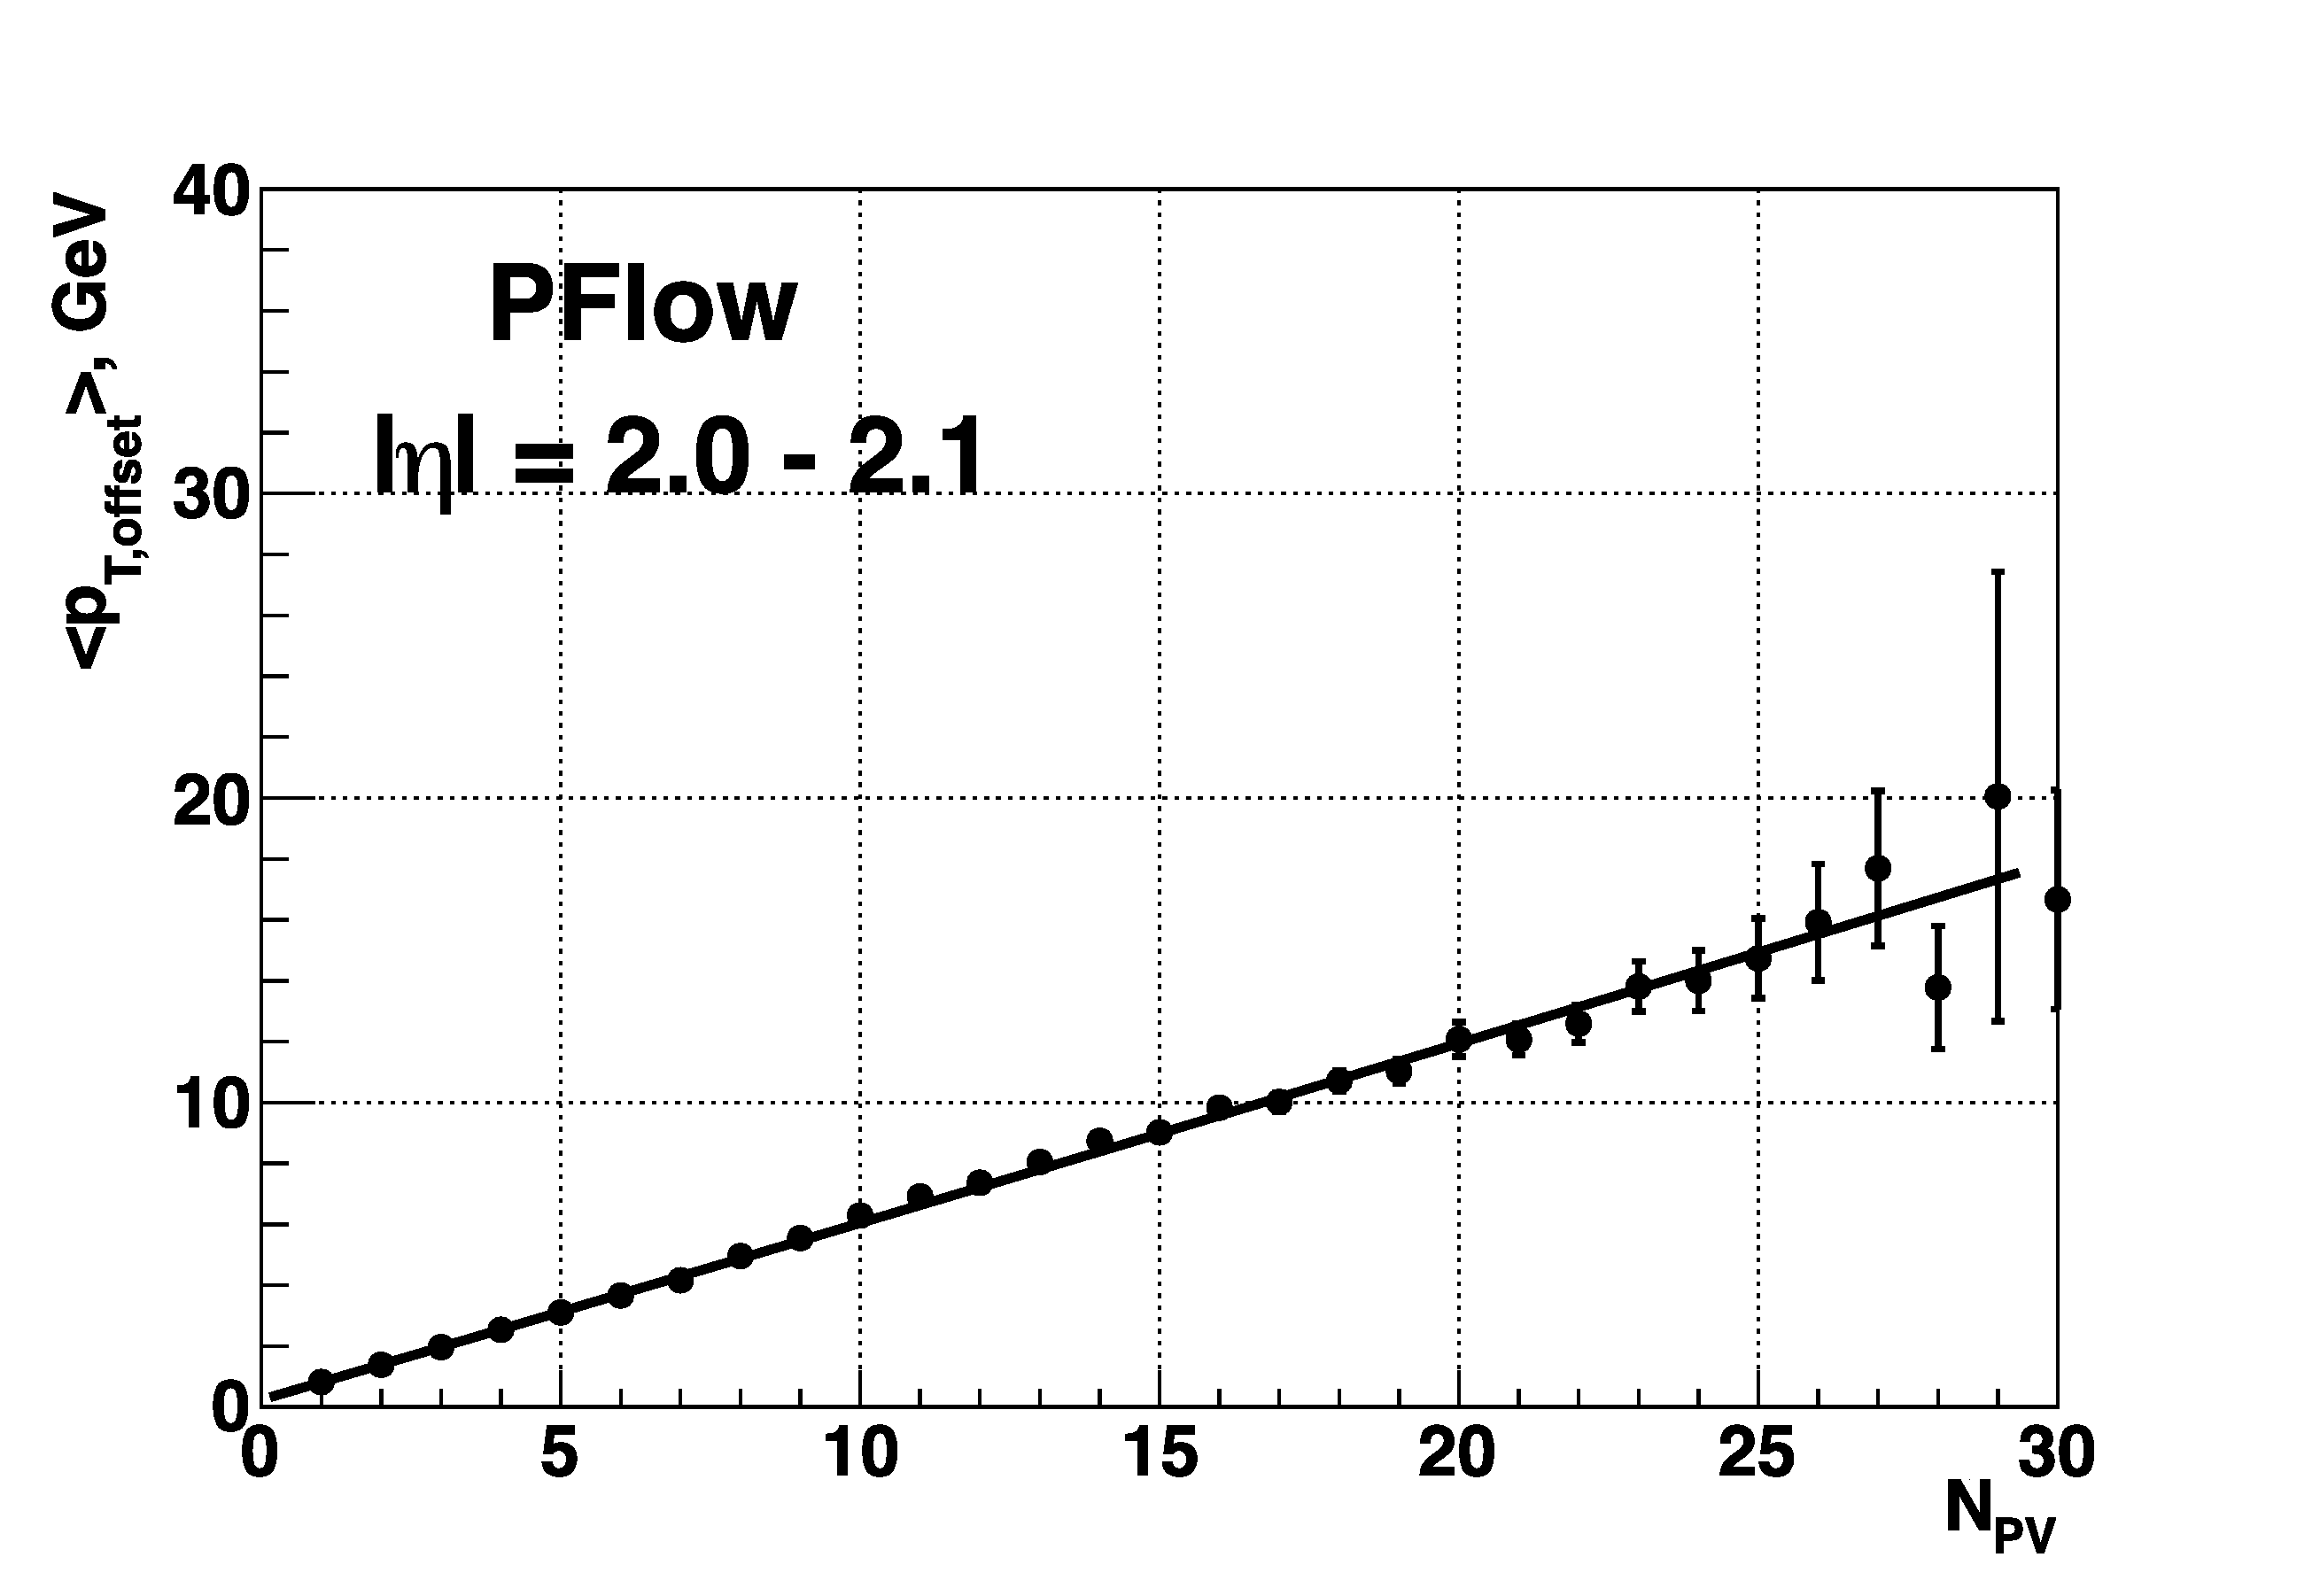
\includegraphics[width=0.45\textwidth]{chapitre4/figs/l1_offset.pdf}} \hfill
  \subcaptionbox{\label{fig:l1_offset_vs_fastjet}}[0.45\textwidth]{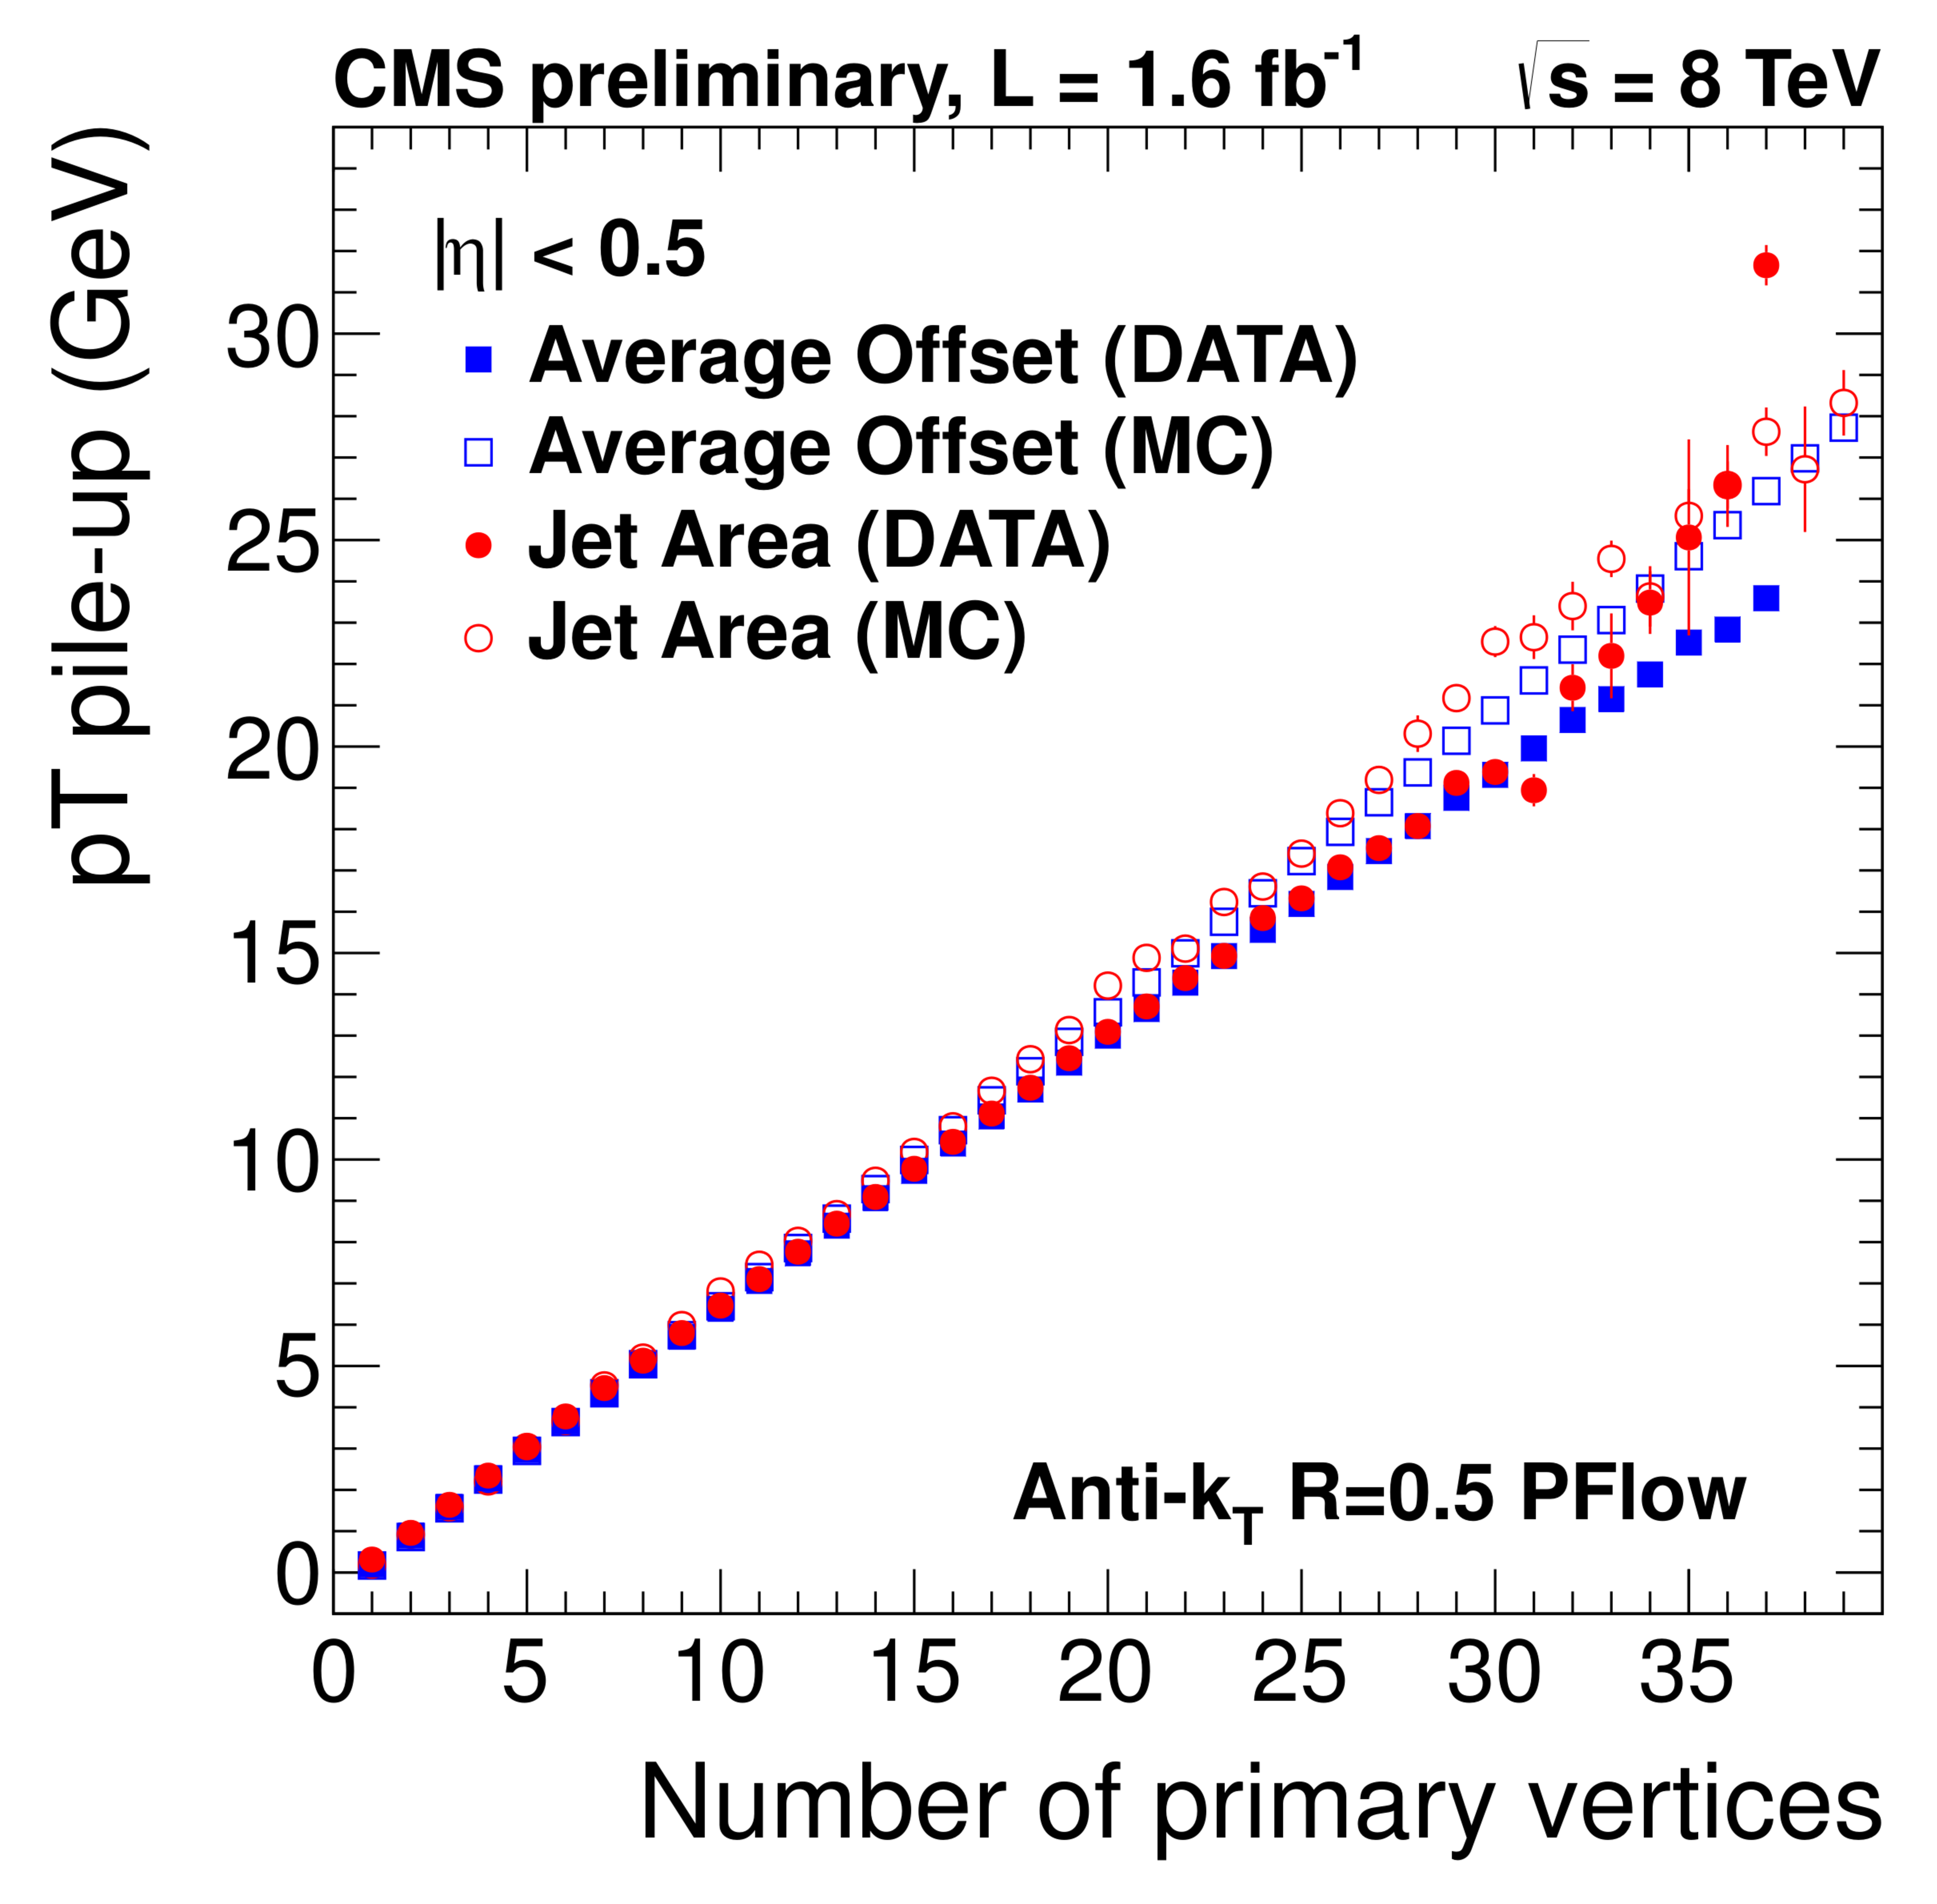
\includegraphics[width=0.45\textwidth]{chapitre4/figs/l1_offset_vs_fastjet.pdf}} \hfill
  \caption{(\subref{fig:l1_offset}) \emph{offset} en fonction du nombre de vertex primaire, pour $\num{2} < \aeta < \num{2.1}$. (\subref{fig:l1_offset_vs_fastjet}) comparaison entre les méthodes \emph{offset} et \emph{fastjet}.}
  \label{fig:jec_l1}
\end{figure}

\subsubsection{La méthode \emph{offset}}

Des événements de biais minimum sont utilisés afin d'estimer l'énergie moyenne portée par un jet à cause du \pu. Cette énergie moyenne est déterminée en fonction du nombre de vertex primaire ($N_{PV}$), une variable directement corrélée au \pu, ainsi qu'en fonction de $\aeta$ (voir \cref{fig:l1_offset}). On obtient ainsi une correction dépendante du nombre de vertex primaires, ainsi que de \aeta. Cette correction est à soustraire de l'énergie du jet afin de supprimer la contribution du \pu.

\subsubsection{La méthode \emph{fastjet}}

Il s'avère que tous les jets ne portent la même énergie due au \pu. La méthode \emph{fastjet} améliore donc la méthode \emph{offset} en ajoutant une dépendance des corrections en fonction de l'aire des jets ($A$) ainsi qu'en fonction de la densité d'énergie ($\rho$), définie comme la médiane de la distribution $p_T^j / A_j$, où $j$ est l'index d'un jet dans l'événement. La correction obtenue est donc dépendante de $\rho$, de $A$ et de \aeta. On présente \cref{fig:l1_offset_vs_fastjet} une comparaison entre ces deux méthodes.

\begin{figure}
  \subcaptionbox{\label{fig:l1_no_corr}}[0.45\textwidth]{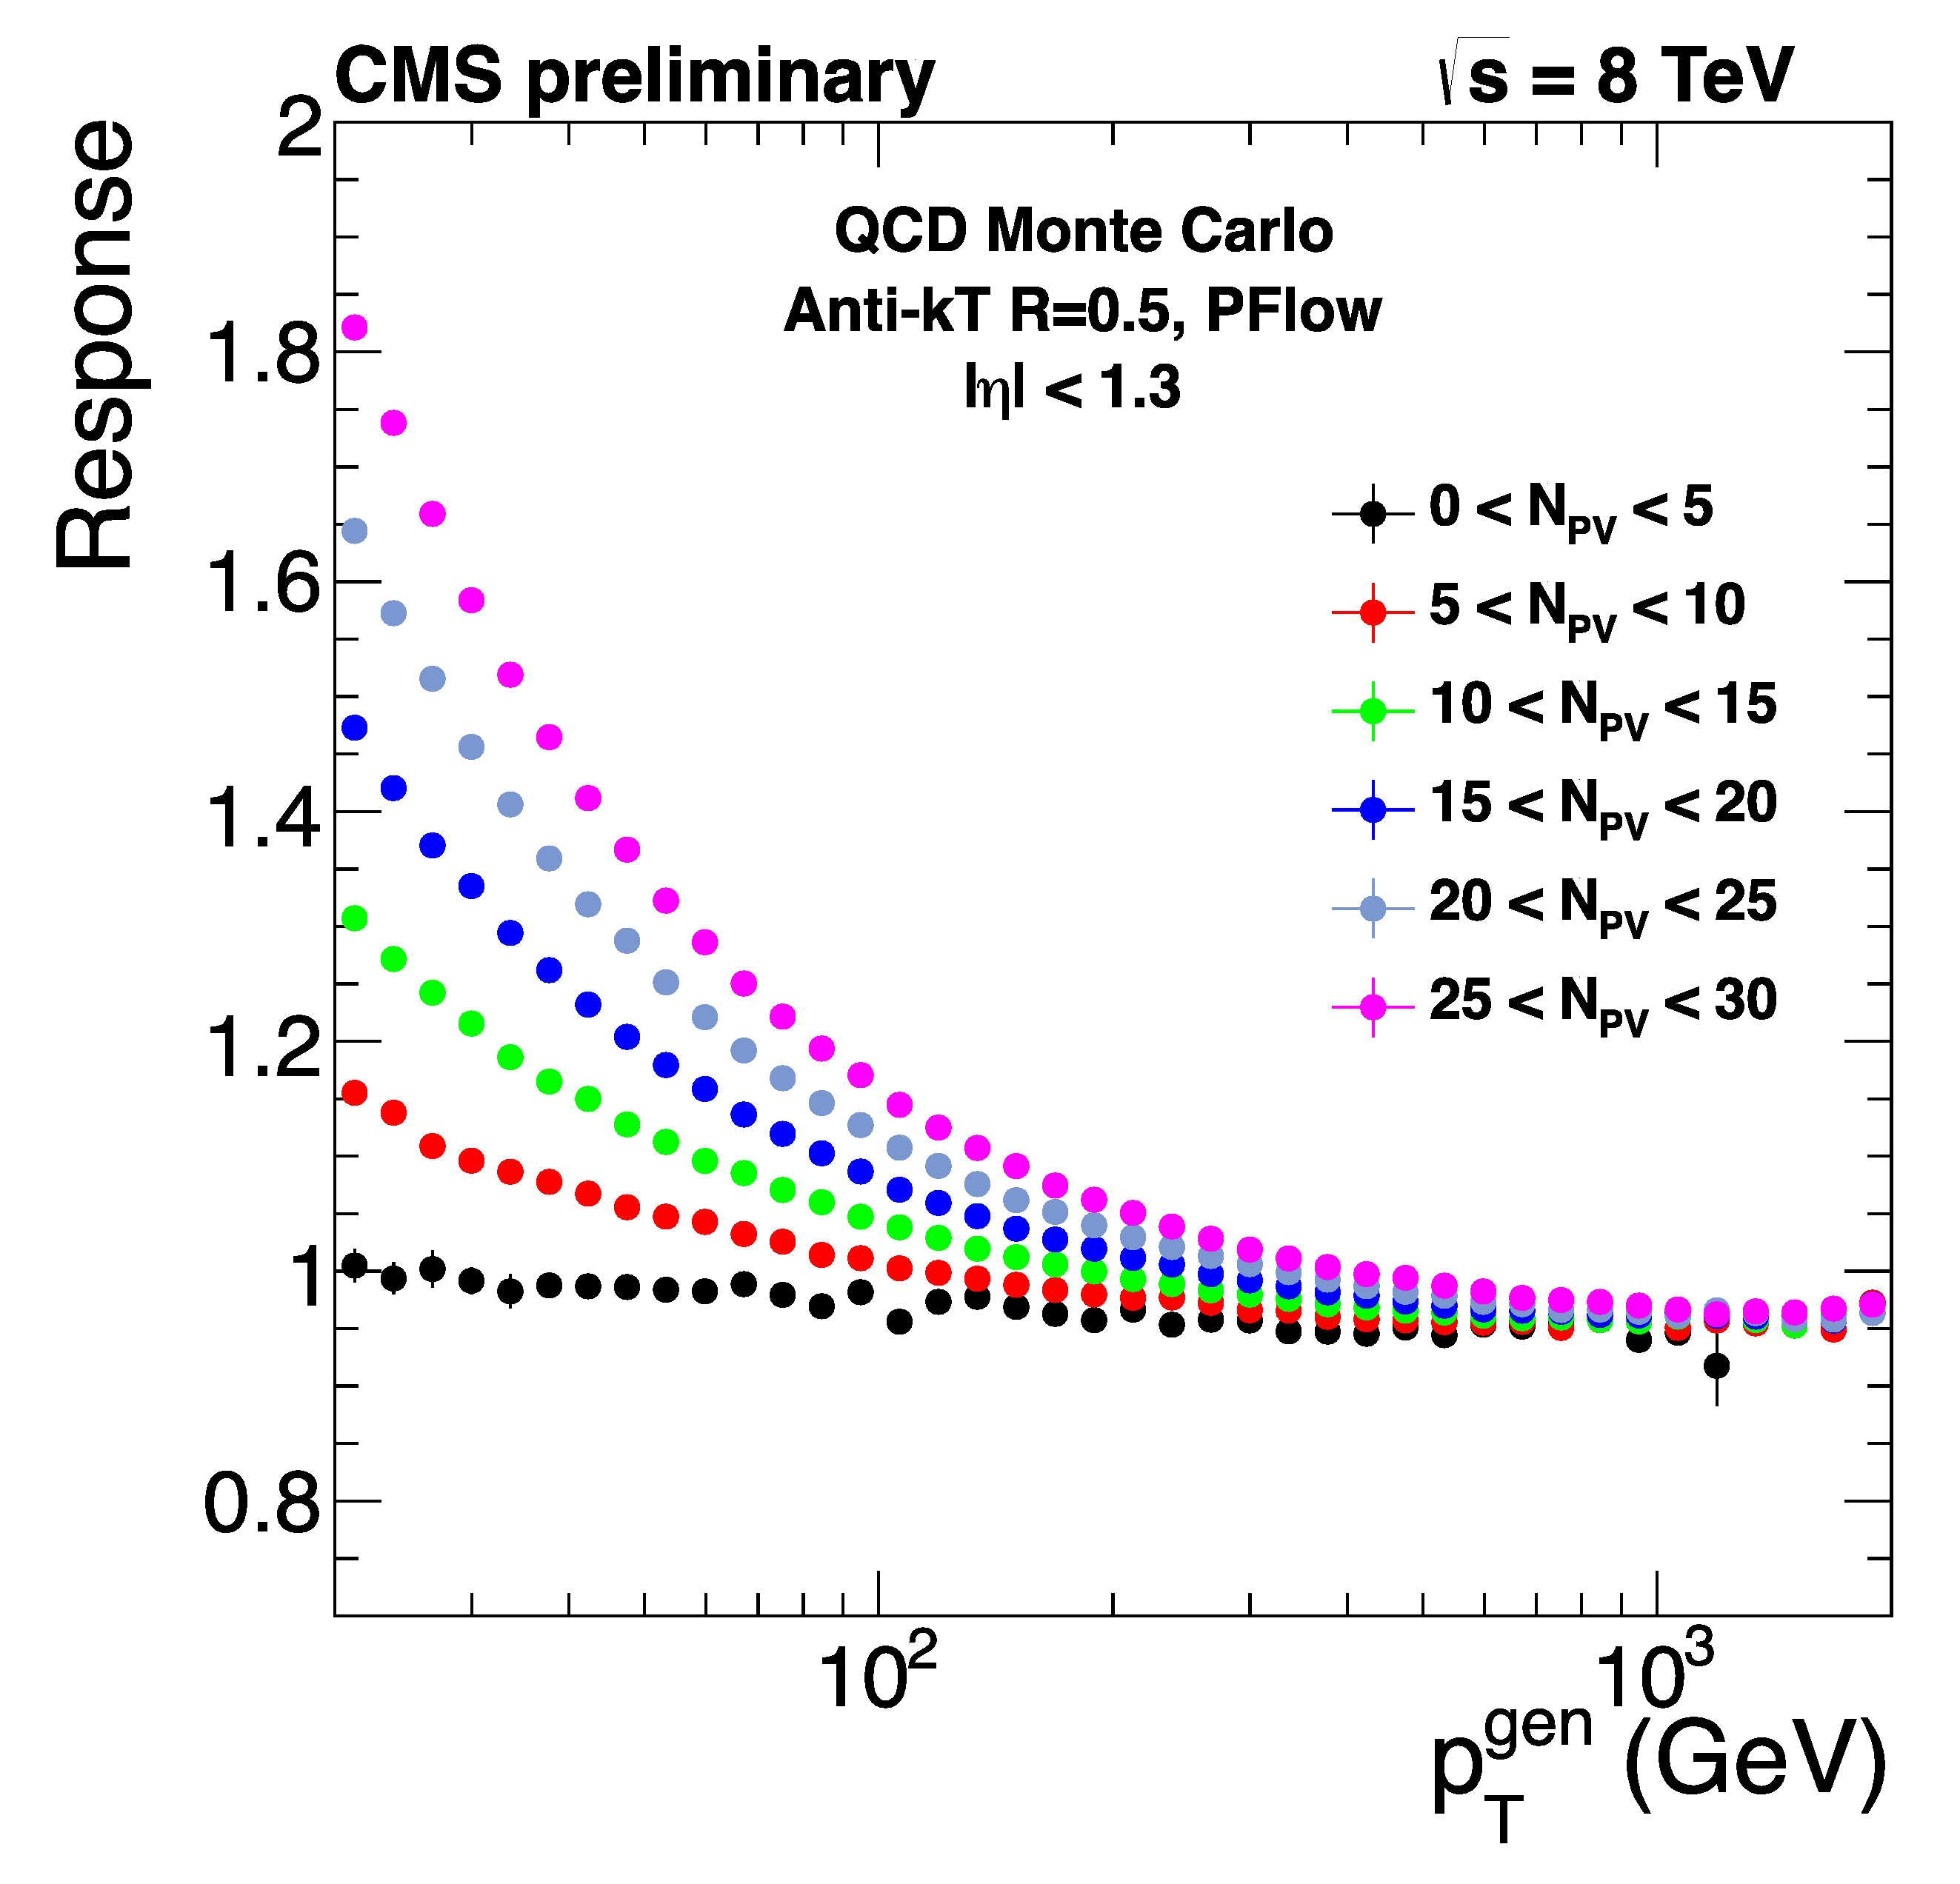
\includegraphics[width=0.45\textwidth]{chapitre4/figs/l1_effect_no_corr.pdf}} \hfill
  \subcaptionbox{\label{fig:l1_with_corr}}[0.45\textwidth]{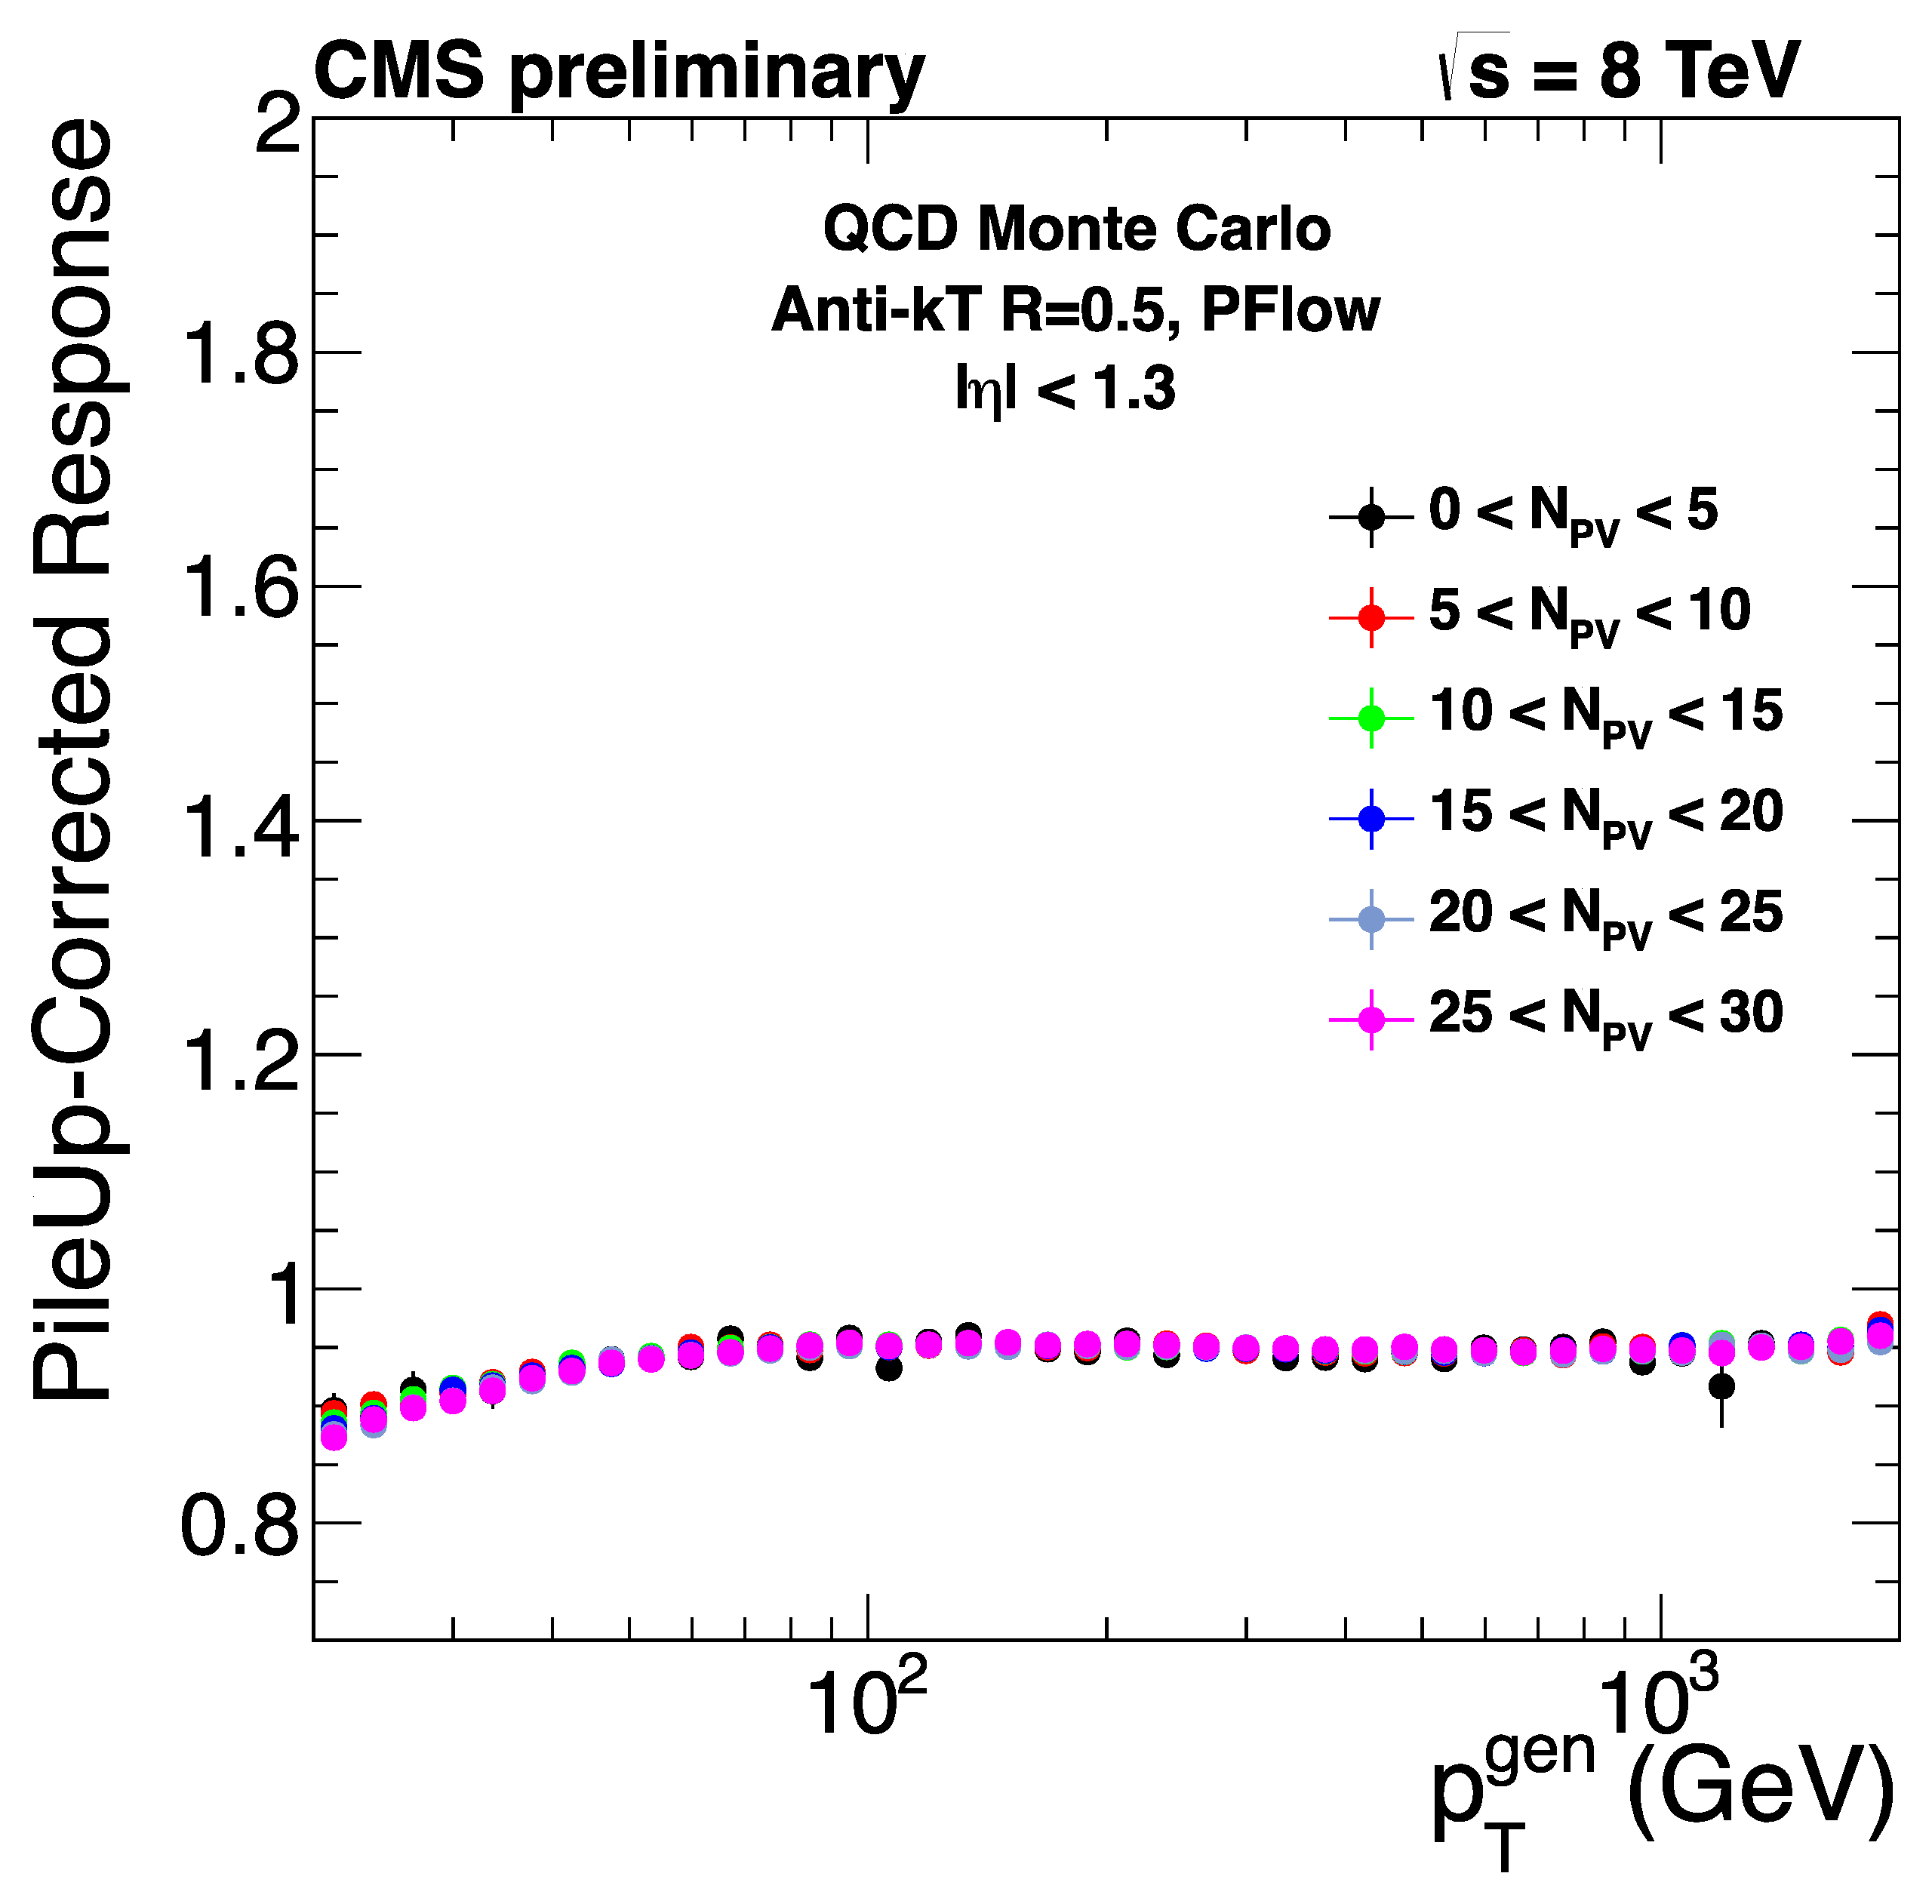
\includegraphics[width=0.45\textwidth]{chapitre4/figs/l1_effect_with_corr.pdf}} \hfill
  \caption{Évolution de la réponse des jets en fonction de l'impulsion transverse simulée, avant l'application des corrections de niveau 1 (\subref{fig:l1_no_corr}) et après (\subref{fig:l1_with_corr}), pour différentes classes de $N_{PV}$.}
  \label{fig:jec_l1_effect}
\end{figure}

\bigskip

Après application des corrections de niveau 1, la réponse des jets, définie comme le rapport en l'impulsion transverse du jet sur l'impulsion transverse vraie, n'est plus dépendante du nombre de vertex primaires, comme on peux le voir \cref{fig:l1_with_corr}.

\subsection{Les corrections de niveau 2 et 3}

Ces corrections sont appliquées après celles de niveau 1. La réponse n'est donc plus dépendante du \pu. Néanmoins, elle varie toujours en fonction de \aeta et du $p_T$. Afin de corriger ces effets, on utilise des événements di-jets, contenant seulement 2 jets. Par conservation de l'impulsion transverse, on a donc $p_T^\text{jet 1} = p_T^\text{jet 2}$. De plus, on considère que les jets dans la région centrale du détecteur ($\aeta < \num{1.3}$) sont correctement reconstruit. On sélection donc des événements avec au moins un jet dans la région centrale, et on calcule la réponse $R$, définie comme $p_T^\text{jet} / p_T^\text{central}$, en fonction de \aeta et $p_T$. Dans le cas d'une reconstruction parfaite, la réponse vaut 1. Dans le cas contraire, le facteur de correction à appliquer est $1 / R$.

%\begin{figure}
  %\subcaptionbox{\label{fig:l2l3_response}}[0.45\textwidth]{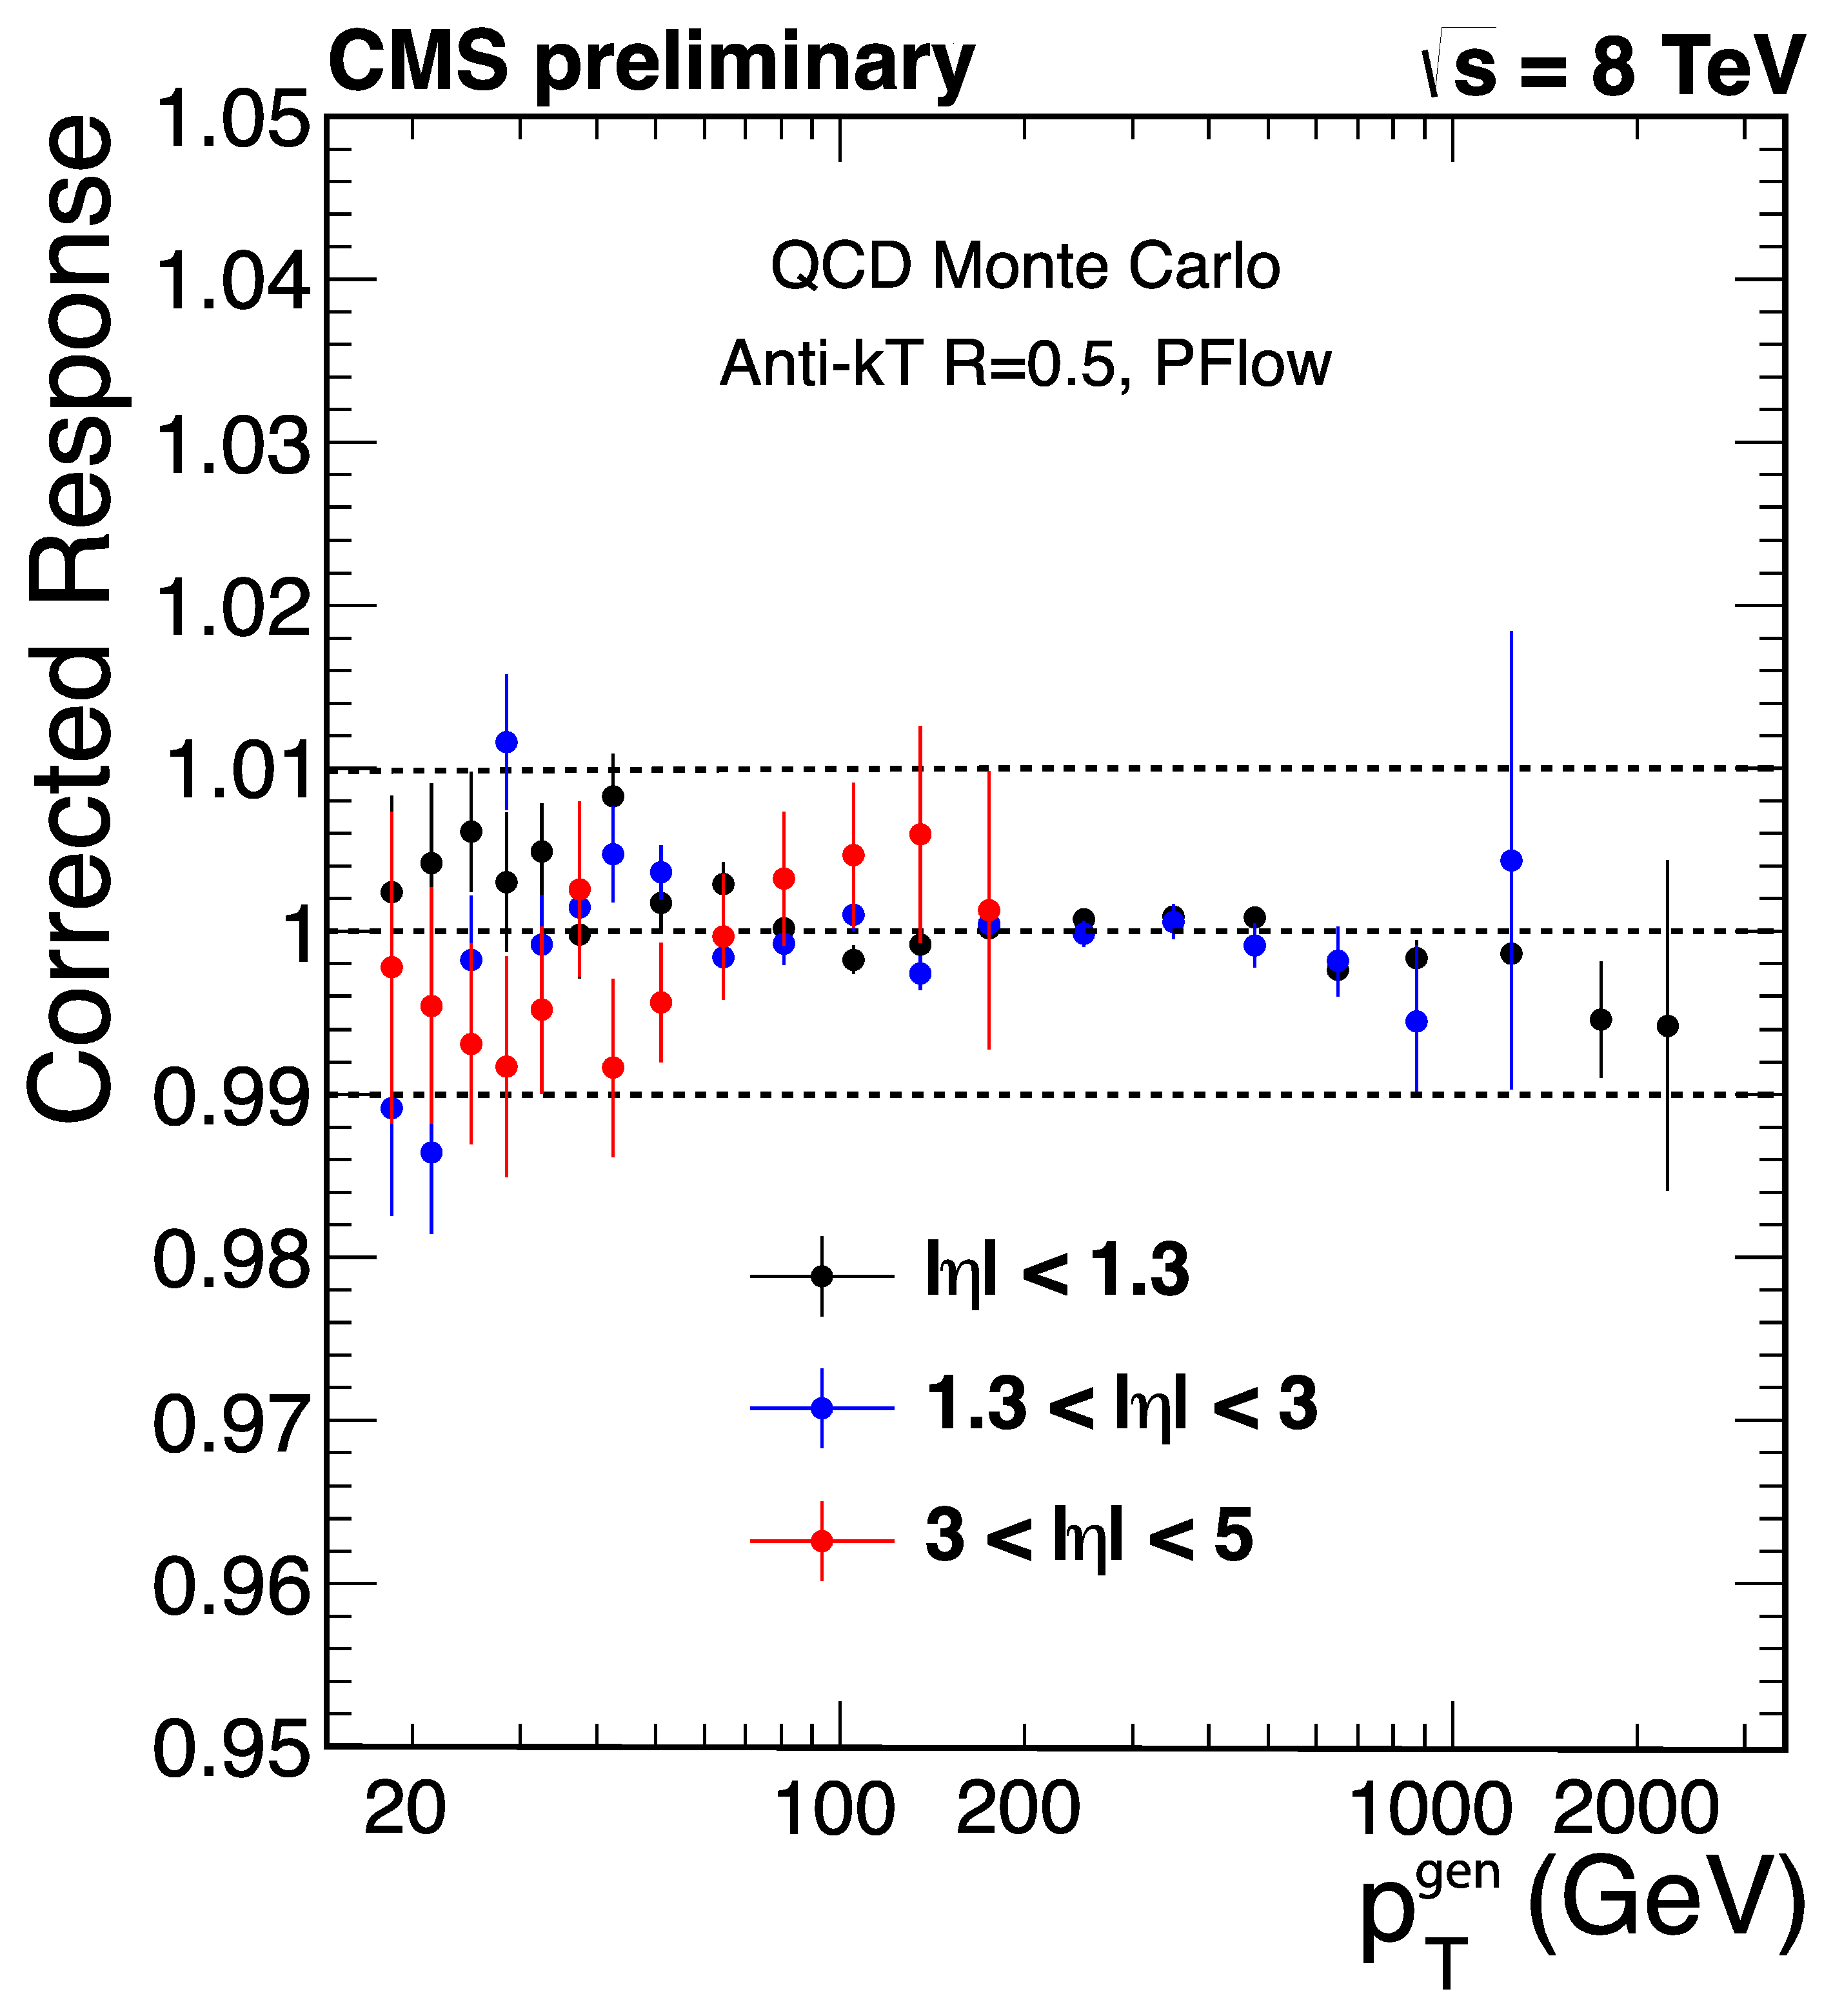
\includegraphics[width=0.45\textwidth]{chapitre4/figs/l2l3_response.pdf}} \hfill
  %\subcaptionbox{\label{fig:l1l2l3}}[0.45\textwidth]{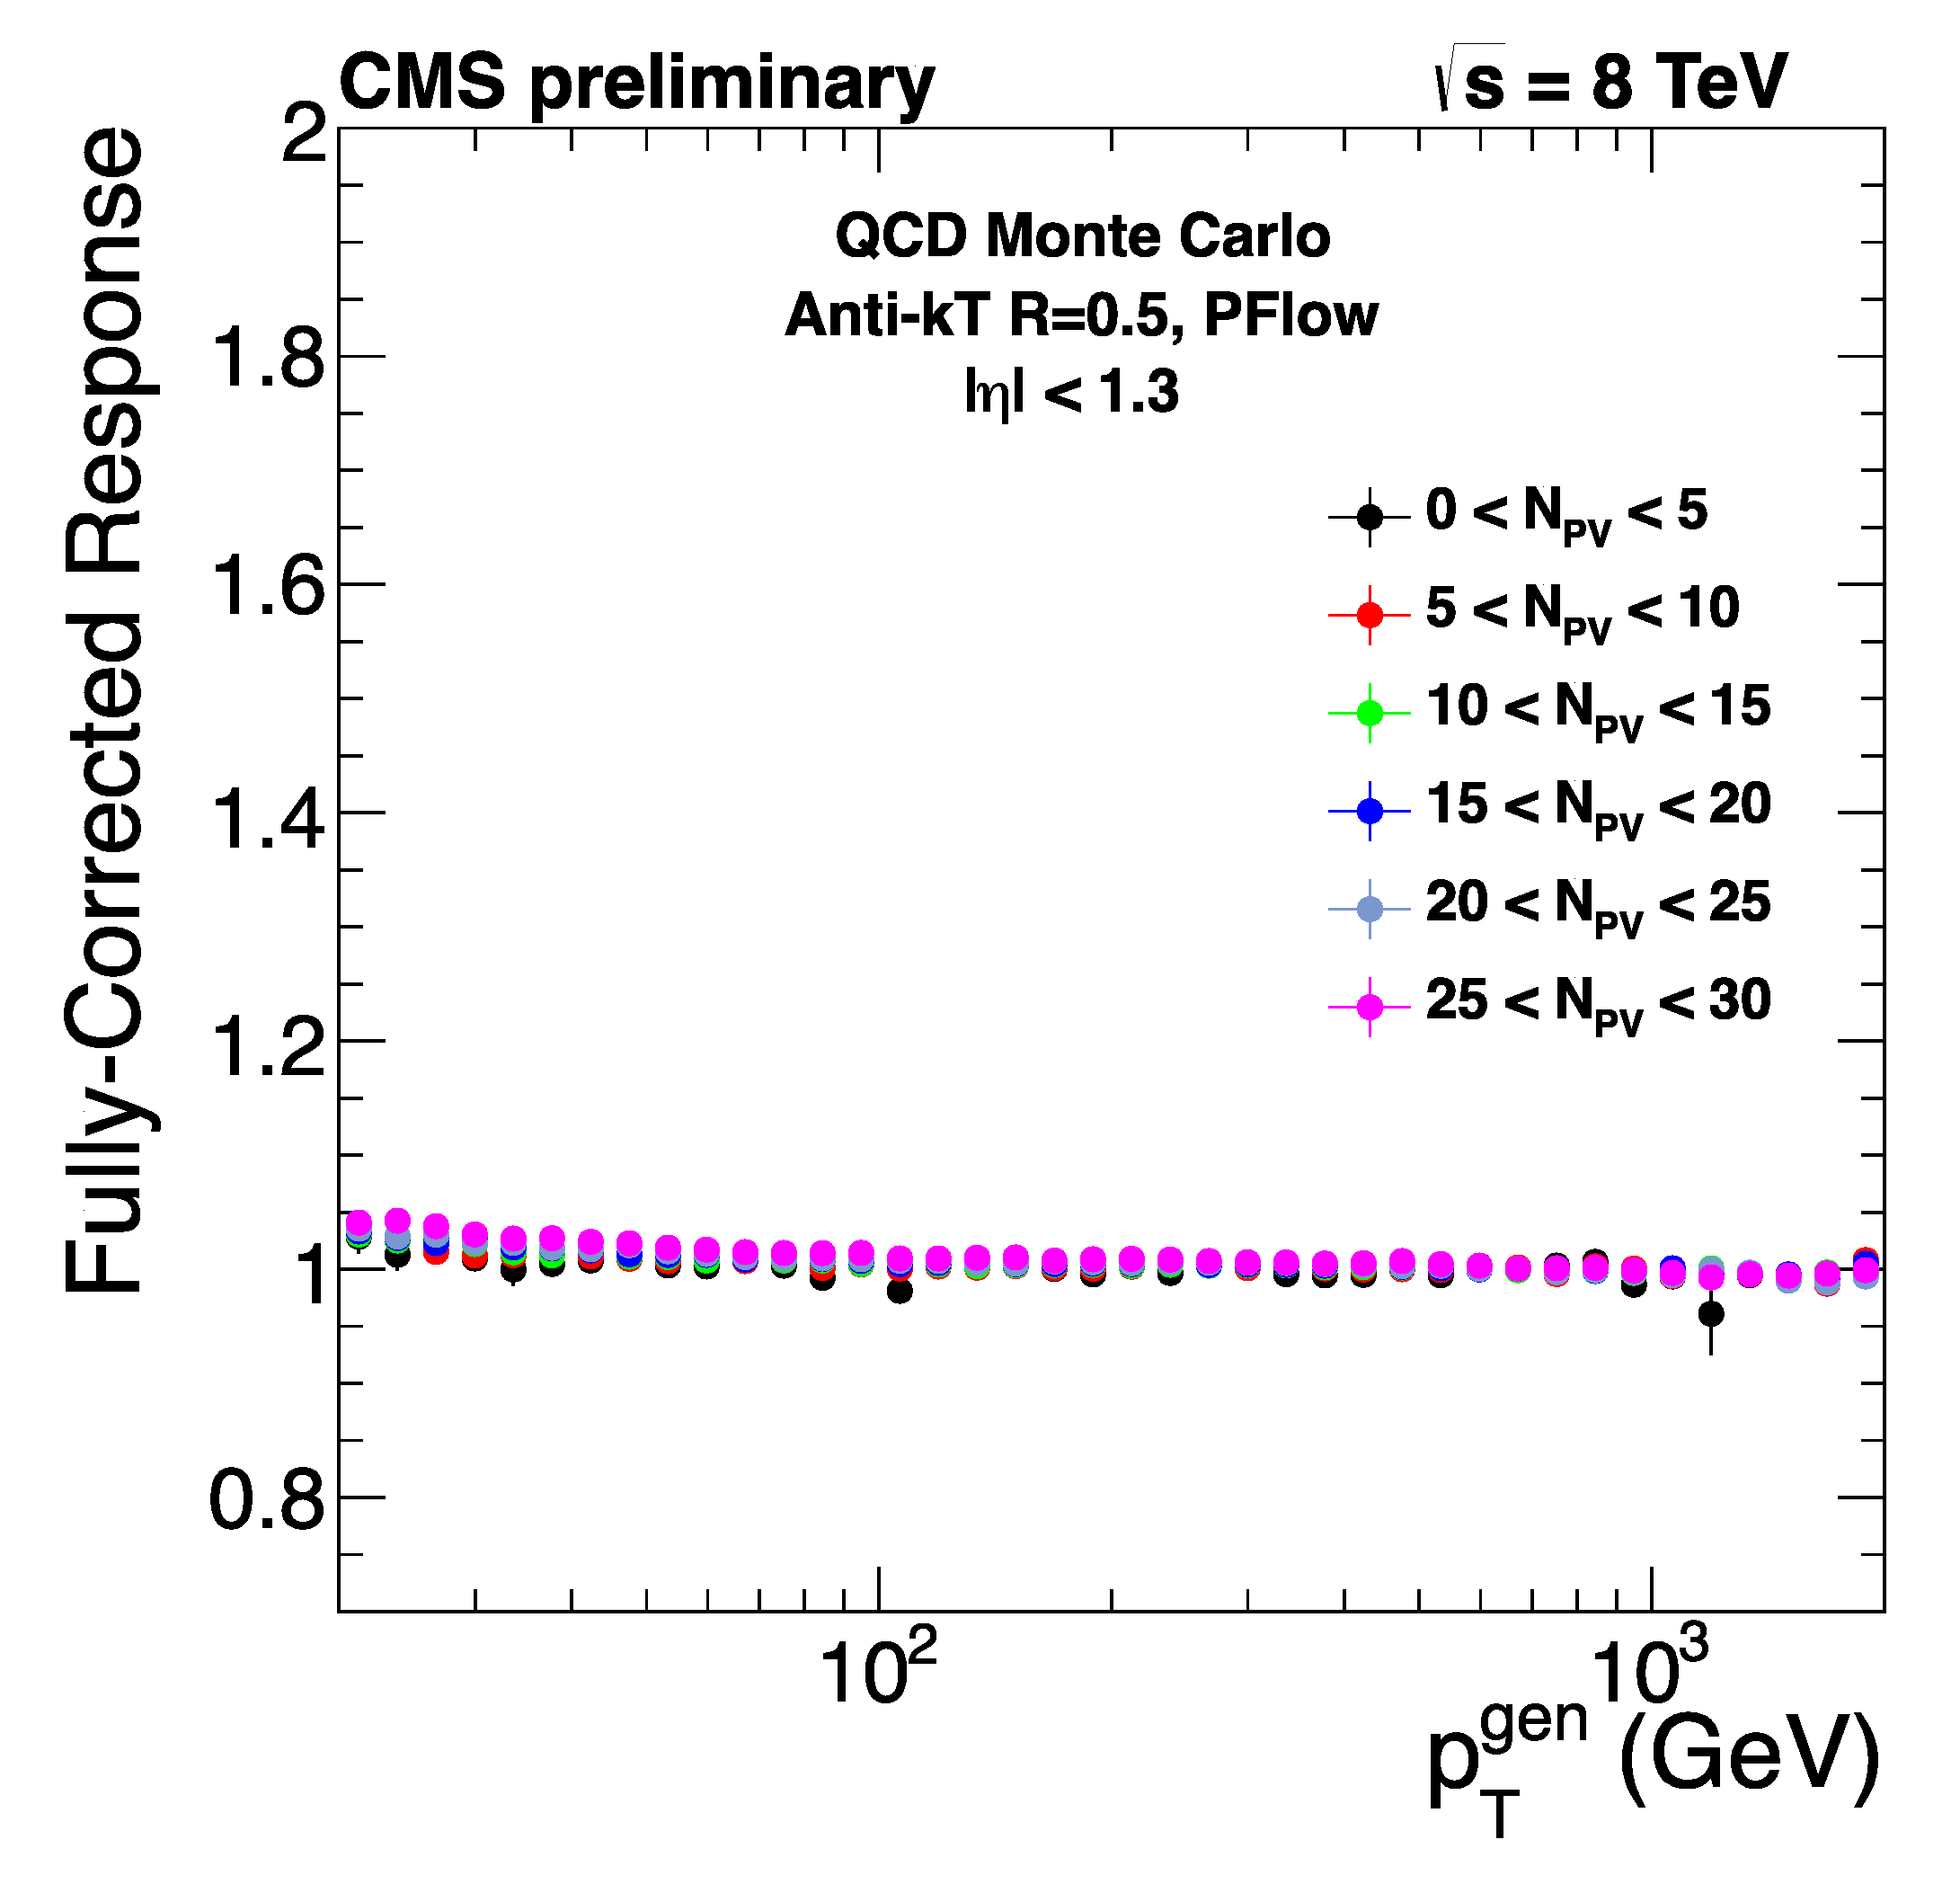
\includegraphics[width=0.45\textwidth]{chapitre4/figs/response_after_l1l2l3.pdf}} \hfill
  %\caption{Évolution de la réponse des jets en fonction de l'impulsion transverse simulée, avant l'application des corrections de niveau 1 (\subref%{fig:l1_no_corr}) et après (\subref{fig:l1_with_corr}), pour différentes classes de $N_{PV}$.}
%  \label{fig:jec_l2l3}
%\end{figure}

\begin{figure}[tbp]
    \centering
    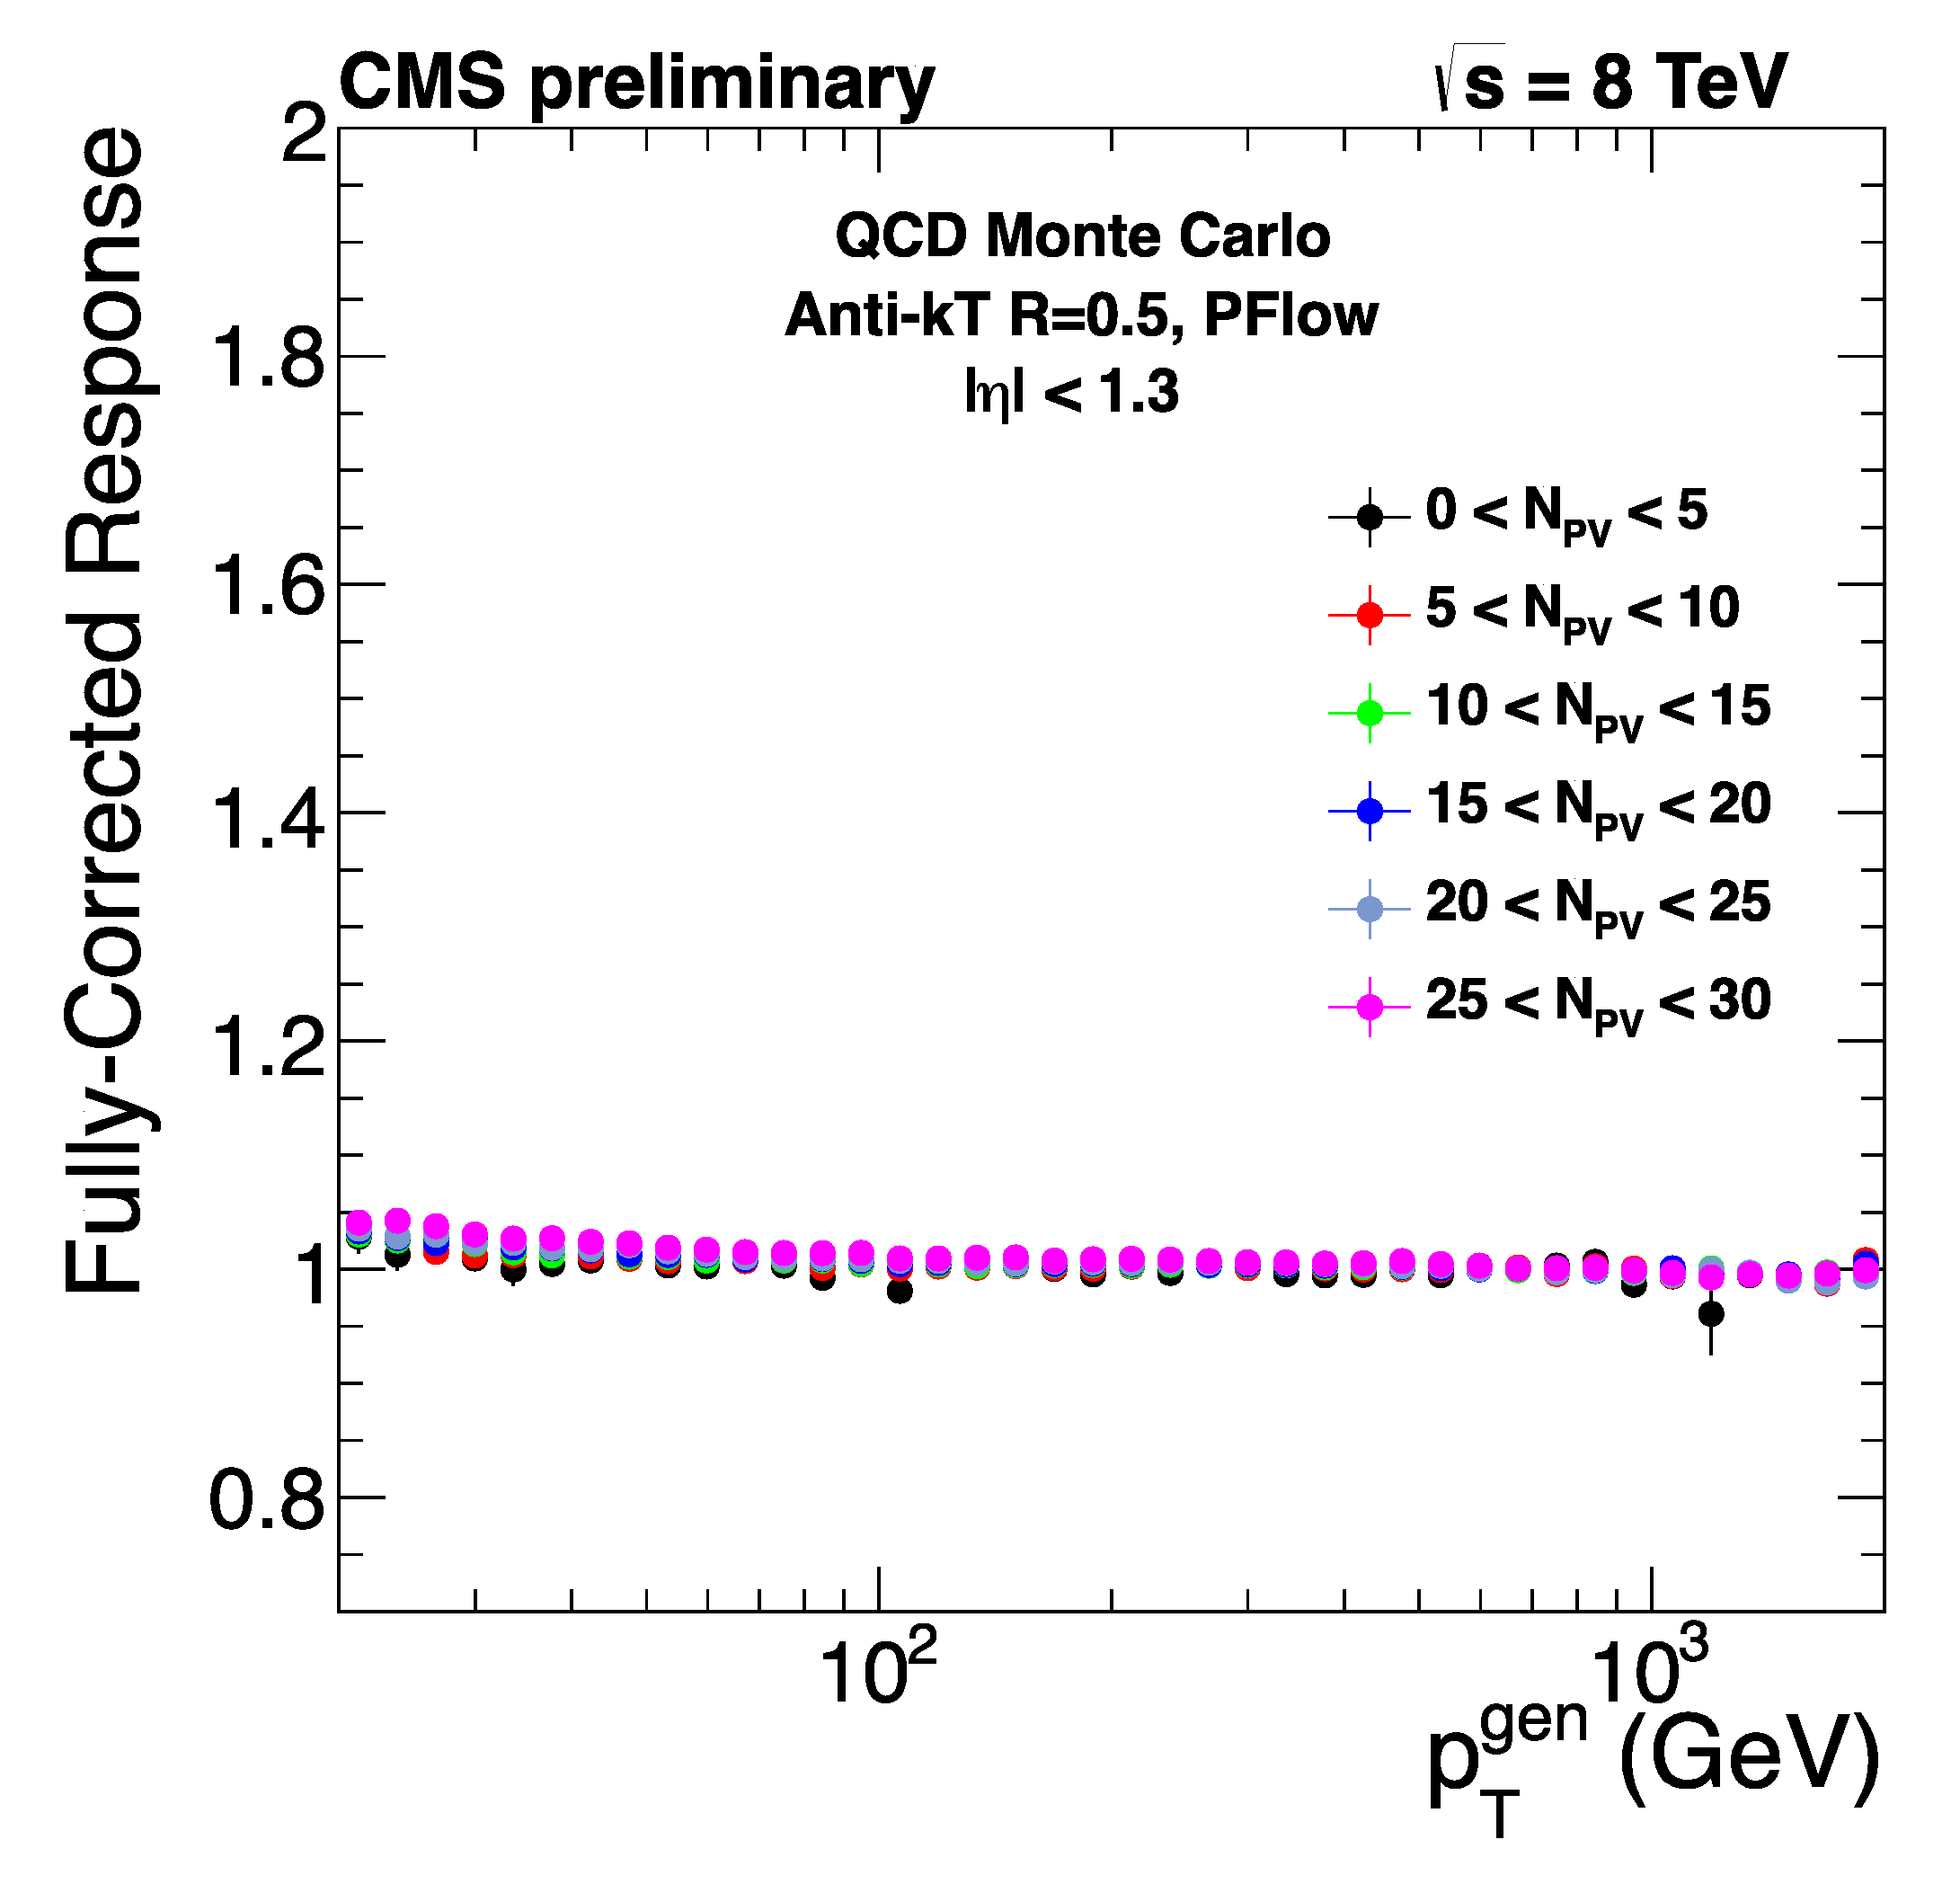
\includegraphics[width=0.55\textwidth]{chapitre4/figs/response_after_l1l2l3.pdf}
    \caption{Réponse des jets après application des corrections de niveau 1, 2 et 3, pour des événements QCD simulés}
    \label{fig:resp_l1l2l3}
\end{figure}

On présente \cref{fig:resp_l1l2l3} la réponse des jets après application des corrections de niveau 1, 2 et 3, pour des événements QCD simulés. La réponse est maintenant linéaire.

\subsection{Les corrections résiduelles}

Les corrections précédentes sont toutes dérivées à l'aide de la simulation. Malheureusement, cette simulation n'est pas parfaite, et des différences existent entre la réponse des jets dans la simulation et dans les données collectées. On applique ainsi un autre niveau de corrections, uniquement sur les données, afin de corriger des dernières différences entre données et simulation. Ces corrections, dépendante de \aeta et du $p_T$ des jets, sont déterminées à l'aide d'événement $\PZ \rightarrow \left[ \Pmuon \APmuon \, | \, \Pelectron \APelectron \right] $ + jets ou $\Pphoton$ + jets.

Ayant fait l'objet de ma tâche de service au sein de CMS, la détermination des corrections résiduelles à l'aide d'événement $\Pphoton$ + jets est décrite en détails dans la section suivante.

\section{Détermination des corrections résiduelles à l'aide d'événements \texorpdfstring{$\Pphoton$}{γ} + jets}

\subsection{Intérêt des événements \texorpdfstring{$\Pphoton$}{γ} + jets}

On cherche à corriger des dernières différences entre simulation et données collectées. Pour cela, on mesure la réponse des jets dans les données, ainsi que dans la simulation, et on corrige les données pour coller à la simulation. Il est donc nécessaire d'utiliser un processus physique qui permet de connaître de façon certain l'énergie d'un jet, sans avoir pour cela à utiliser la vérité de la simulation.

\begin{figure}[t!] \centering
  \subcaptionbox{\label{fig:g_plus_jet_1}}[.4\linewidth]{
  \begin{fmfgraph*}(180,120)
    \fmfpen{0.5}
    \fmfleft{i1,i2}
    \fmfright{o1,o2}
    \fmf{gluon}{i1,v1}
    \fmf{fermion}{i2,v1}
    \fmf{fermion,label=\Pquark}{v1,v2}
    \fmf{fermion}{v2,o1}
    \fmf{photon}{v2,o2}
    \fmffreeze
    \fmfdot{v1,v2}
    \fmflabel{\Pquark}{i2}
    \fmflabel{\Pquark}{o1}
    \fmflabel{\Pphoton}{o2}
  \end{fmfgraph*}}\qquad \quad%
  % \begin{fmfgraph*}(180,120)
  %   \fmfpen{0.5}
  %   \fmfleft{i1,i2}
  %   \fmfright{o1,o2,o3}
  %   \fmf{gluon}{i2,v1}
  %   \fmf{gluon}{v3,o1}
  %   \fmf{fermion}{i1,v3}
  %   \fmf{fermion,label=\APquark}{v3,v2,v1}
  %   \fmf{fermion}{v1,o3}
  %   \fmffreeze
  %   \fmf{photon,label=\Pphoton}{v2,o2}
  %   \fmfdot{v1,v2,v3}
  %   \fmflabel{\Pquark}{i1}
  %   \fmflabel{\Pquark}{o3}
  % \end{fmfgraph*}}\qquad \quad%
  \subcaptionbox{\label{fig:g_plus_jet_2}}[.4\linewidth]{
  \begin{fmfgraph*}(180,120)
    \fmfpen{0.5}
    \fmfstraight
    \fmfleft{i1,i2}
    \fmfright{o1,o2,o3}
    \fmf{fermion}{i1,v1,i2}
    \fmf{fermion}{v4,v2}
    \fmf{phantom}{o1,v4}
    \fmf{fermion,label=\Pquark}{v2,v3}
    \fmf{photon,label=$\Pphoton$}{v3,o3}
    \fmf{gluon}{v1,v2}
    \fmffreeze
    \fmf{fermion}{v3,o2}
    \fmfdot{v1,v2,v3}
    \fmflabel{\APquark}{i2}
    \fmflabel{\Pquark}{i1}
    \fmflabel{\Pquark}{o2}
    \fmflabel{\APquark}{v4}
  \end{fmfgraph*}
  }
  \caption{Diagrammes de Feynman associés à la production d'un photon et d'un jet (\subref{fig:g_plus_jet_1}) et d'un photon et de deux jets (\subref{fig:g_plus_jet_2}).}
  \label{fig:gamma_jet_diagrams}
\end{figure}

On utilise des processus comportant uniquement deux particules dans l'état final : une particule dont on connaît très bien les propriétés (boson \PZ, photon, \ldots), qui sera notre sonde, et un jet. On utilise ensuite les propriétés de la sonde pour déterminer celles du jet. Dorénavant, on se concentrera uniquement sur les événements \Pphoton + jets.

\bigskip

On présente \cref{fig:gamma_jet_diagrams} deux diagrammes de Feynman représentant la production d'un photon accompagné d'un ou deux jets. L'impulsion dans le plan transverse étant nulle au moment de la collision, on a, dans l'état final
\begin{align*}
  \vec{p}_T &= 0 = \vec{p}_{T}^{\Pphoton} + \vec{p}_T^\text{jet}\\
  \norm{\vec{p}_T^{\Pphoton}} &= \norm{\vec{p}_T^{jet}}
\end{align*}

Ainsi, il est suffisant de connaître l'impulsion transverse de la sonde pour déterminer l'impulsion transverse du jet. Le calorimètre électromagnétique étant bien plus performant que le calorimètre hadronique, on voit ici tout l'intérêt du choix du photon comme sonde.

\subsection{Détermination de la réponse des jets}

On cherche à déterminer la réponse $R$ des jets
%c'est-à-dire le rapport $R = p_T^\text{jet} / p_T^{\Pphoton}$
, qui tend vers 1 si l'on reconstruit parfaitement le jet. On utilise deux méthodes différentes pour déterminer cette réponse : la méthode de la balance, et la méthode MPF, détaillée ci-dessous.

\subsubsection{La méthode de la balance}

On utilise le principe de conservation de l'impulsion transverse. On a alors
\begin{align*}
  \norm{\vec{p}_T^{\Pphoton}} &= \norm{\vec{p}_T^{jet}}
\end{align*}
et on défini la réponse $R$ par la relation
\begin{align*}
    R &= \frac{p_T^\text{jet}}{p_T^{\Pphoton}}
\end{align*}

Cette méthode est très simple et performante. Néanmoins, elle est très sensible au \pu, ainsi qu'aux radiations dans l'état final. En effet, la présence d'autres jets dans l'état final vont venir perturber la balance entre le jet et le photon. On verra par la suite comment restaurer cette balance.

\subsubsection{La méthode MPF (\emph{Missing $E_T$ projection fraction})}

Un événement \Pphoton + jets n'a pas de \met. Ainsi, au niveau partonique, on a
\begin{align*}
  \vec{p}_T^{\Pphoton} + \vec{p}_T^{\text{recul}} &= -\vec{\met} = \vec{0}
\end{align*}
où $\vec{p}_T^{\text{recul}}$ est le vecteur impulsion transverse de tous les autres particules dans l'événement.

Après reconstruction, on a
\begin{align*}
  R_{\Pphoton} \, \vec{p}_T^{\Pphoton} + R_{\text{recul}} \, \vec{p}_T^{\text{recul}} &= -\vec{\met}
\end{align*}
$R_X$ désigne ici la réponse des détecteurs lors de la reconstruction de l'objet $X$.

On considère que les photons sont reconstruits de façon parfaite, on pose donc $R_{\Pphoton} = 1$. En utilisant le fait que $\vec{p}_T^{\text{recul}} = -\vec{p}_T^{\Pphoton}$ on obtient
\begin{align*}
  R_{\text{recul}} &= 1 + \frac{\vec{\met} \cdot \vec{p}_T^{\Pphoton}}{\left( p_T^{\Pphoton} \right)^2} \equiv R_{\text{MPF}}
\end{align*}

Cette méthode n'est pas dépendante de la présence de jets additionnels dans l'événement, mais requiert par contre une excellente reconstruction de l'énergie transverse manquante. C'est le cas dans CMS grâce à l'utilisation de l'algorithme du \pf.

\medskip

Cette méthode est utilisée pour produire les corrections officielles. La méthode de la balance permet de vérifier la compatibilité des corrections obtenues.

\end{fmffile}